\begin{enumerate}
\item  Les supports $\mathcal{C}_{\alpha }$ et $\mathcal{C}_{\alpha +\pi }$ des courbes param{\'e}tr{\'e}es sont {\'e}gaux car 
\begin{displaymath}
r_{\alpha}(t)=r_{\alpha +\pi }(t) 
\end{displaymath}
D'autre part, $\mathcal{C}_{-\alpha }=s_{Oy}(\mathcal{C}_{\alpha })$ car $r_{-\alpha }(t)=-r_{\alpha }(-t)$.

\item  Comme $r(t+3\pi )=-r(t)$ la param{\'e}trisation est $3\pi $ p{\'e}riodique.\newline
Le $\cos $ du d{\'e}nominateur s'annule lorsque 
\begin{displaymath}
 t\equiv \frac{3\pi }{4} \hspace{1cm} (\frac{3\pi }{2})
\end{displaymath}
Un intervalle de longueur $3\pi $ contient donc trois valeurs de $t$ annulant le $\cos $.\newline
Le $\sin $ s'annule lorsque 
\begin{displaymath}
 t\equiv 3\alpha \hspace{1cm} (3\pi)
\end{displaymath}
Un intervalle de longueur $3\pi $ contient donc une seule valeur de $t$ annulant le $\sin $.\newline
Comme $\alpha \in \left[ 0,\frac{\pi }{2}\right] $ choisissons $\left[ 0,3\pi\right] $ comme intervalle pour d'étude $t$. Il y a alors trois branches infinies pour les valeurs suivantes du paramètre
\begin{align*}
 \frac{3\pi }{4} & &
 \frac{9\pi }{4}=\frac{\pi}{4}+2\pi & &
3\alpha 
\end{align*}
\begin{itemize}
\item  En $\frac{3\pi }{4}$. Comme
\begin{displaymath}
 \cos \frac{2t}{3} = \sin (\frac{\pi }{2}-\frac{2t}{3})
 = \sin (\frac{2}{3}(\frac{3\pi }{4}-t))
 \sim \frac{2}{3}(\frac{3\pi }{4}-t)
\end{displaymath}
On d{\'e}duit que $r(t)\sin (t-\frac{3\pi }{4})$ diverge vers $+\infty $ ou $-\infty $ d'un c{\^o}t{\'e} ou de l'autre de $\frac{3\pi }{4}$.\newline
Il n'y a donc pas d'asymptote mais seulement une branche parabolique de direction asymptotique
\begin{displaymath}
 \overrightarrow{u}_{\frac{3\pi }{4}}
\end{displaymath}

\item  En $\frac{9\pi }{4}=\frac{\pi }{4}+2\pi $. La situation est analogue.\newline
Il n'y apas d'asymptote mais une branche parabolique de direction asymptotique
\begin{displaymath}
 \overrightarrow{u}_{\frac{\pi }{4}}
\end{displaymath}

\item  En $3\alpha $. On a en revanche 
\begin{displaymath}
 \sin (t-3\alpha )=\sin (3(\frac{t}{3} -\alpha ))\sim 3(\frac{t}{3}-\alpha ) 
\Rightarrow \rho (t)\sin (\frac{t}{3}-\alpha )\sim \frac{3a\cos \alpha }{\cos ^{2}2\alpha }
\end{displaymath}
Il existe donc une asymptote.\newline
Pour étudier la position de la courbe par rapport {\`a} l'asymptote, posons 
\begin{displaymath}
u=\frac{t}{3}-\alpha  
\end{displaymath}
et formons un d{\'e}veloppement limit{\'e} de $r(t)\sin (t-3\alpha )$ suivant $u$. On obtient
\begin{displaymath}
 \frac{a\cos \alpha \sin 3u}{\cos ^{2}(2\alpha +2u)\sin u} 
= 3a\frac{\cos \alpha }{\cos ^{2}2\alpha } + \left( 12a\frac{\cos \alpha }{\cos ^{3}2\alpha }\sin 2\alpha \right) u+u\epsilon (u)
\end{displaymath}
On en d{\'e}duit que la courbe est, suivant le signe de $u$, d'un c{\^o}t{\'e} ou de l'autre de l'asymptote. On remarque aussi que le coefficient de $u$ change de signe lorsque $\alpha $ traverse la valeur $\frac{\pi }{4}$ pour laquelle il n'y a pas d'asymptote.
\end{itemize}

\begin{figure}[ht]
  \centering
  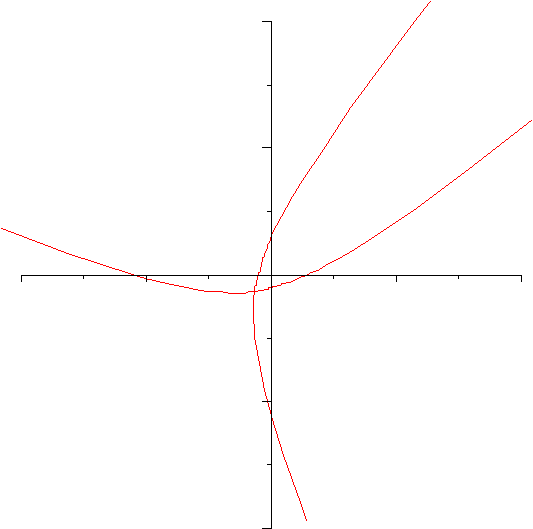
\includegraphics[width=9cm]{Ccurv1_1.pdf}
  \caption{Tracé de $\mathcal C_\frac{\pi}{4}$pour $a=1$}
  \label{fig:Ccurv1_1}
\end{figure}
\item  Le trac{\'e} de la courbe (Fig. \ref{fig:Ccurv1_1}) se fait {\`a} la machine en remarquant que $r(t)$ est n{\'e}gatif dans $\left[0,\frac{3\pi }{4}\right] $ et positif dans $\left[ \frac{3\pi }{4},3\pi \right] $. Le changement
de signe se fait "{\`a} l'infini". La courbe ne passe pas par l'origine.\newline
Comme $\alpha =\frac{\pi }{4}$, $3\alpha =\frac{3\pi }{4}$, il n'y a donc pas d'asymptote mais seulement deux branches paraboliques.

\item Un point est birégulier lorsque la vitesse et l'accélération en ce point forment une famille libre.\newline Notons $f$ la paramétrisation, exprimons la vitesse et l'accélération puis le déterminant :
\begin{align*}  
 f(t) =& 0 + r(t) \overrightarrow e_t \\
 \overrightarrow f'(t) =& r'(t) \overrightarrow e_t +r(t) \overrightarrow e_{t+\frac{\pi}{2}} \\
\overrightarrow f''(t) =& (r''(t) -r(t))\overrightarrow e_t + 2r'(t) \overrightarrow e_{t+\frac{\pi}{2}} \\
\det(\overrightarrow f'(t),\overrightarrow f''(t)) =&
\begin{vmatrix}
 r'(t) & r''(t) -r(t)  \\
 r(t) & 2r'(t)
\end{vmatrix}
\end{align*}
La condition assurant la non bir{\'e}gularit{\'e} s'{\'e}crit donc
\begin{displaymath}
 2r'^2 -rr''+r^2=0
\end{displaymath}
En posant $\lambda =\frac{1}{r}$, cette condition devient 
\begin{displaymath}
\lambda +\lambda ''=0 
\end{displaymath}
Pour l'exprimer simplement dans le cas particulier qui nous est demandé, on commence par lin{\'e}ariser $\lambda $. Il vient
\begin{displaymath}
\lambda  = \frac{1}{2}\sin (\frac{t}{3}-\alpha ) 
+ \frac{1}{4}\sin (\frac{5t}{3}-\alpha )
-\frac{1}{4}\sin (t+\alpha )
\end{displaymath}
puis
\begin{multline*}
\lambda +\lambda'' = \frac{1}{2}(1-\frac{1}{9})\sin (\frac{t}{3}-\alpha )+\frac{1}{4}(1-\frac{25}{9})\sin (\frac{5t}{3}-\alpha ) \\
 = \frac{4}{9}\sin (\frac{t}{3}-\alpha )-\frac{4}{9}\sin (\frac{5t}{3}-\alpha ) 
 = -\frac{8}{9}\cos (t-\alpha )\sin (\frac{2t}{3})
\end{multline*}
Cette expression est nulle lorsque 
\begin{displaymath}
t-\alpha \equiv \frac{\pi }{2} \hspace{1cm} (\pi)  
\end{displaymath}
Lorsque $\alpha $ varie le point tel que $t-\alpha \equiv \frac{\pi }{2}$ modulo $\pi$ d{\'e}crit la courbe param{\'e}tr{\'e}e
\[
r(t)=-\frac{a\sin t}{\cos ^{3}\frac{2t}{3}}
\]
\end{enumerate}
